\section{Testing WebRTC}

\thispagestyle{empty}

In this chapter we will study how WebRTC performs in different use cases and topologies previously described in chapter~\ref{sec:topologies}. All tests will be done using a real working environment with the tools previously mentioned in chapter~\ref{sec:testingEnv}.

\subsection{Point-to-point}

In a point-to-point scenario we have performed different tests to calculate how the application performs. 

\subsubsection{WiFi scenario}

Firstly we have stablished a simple call between two peers that handle video and audio in an open WiFi network. This network does not carry any UDP packet filter or Firewall, the connection is performed without the need of STUN or TURN, we could easily say it is a straight forward peer-to-peer connection. The aim of this test is to observe how the captures differ between origin and receiver on the {\it StatsAPI} and {\it ConMon} layer.

 \begin{figure}[h]
  \centering
    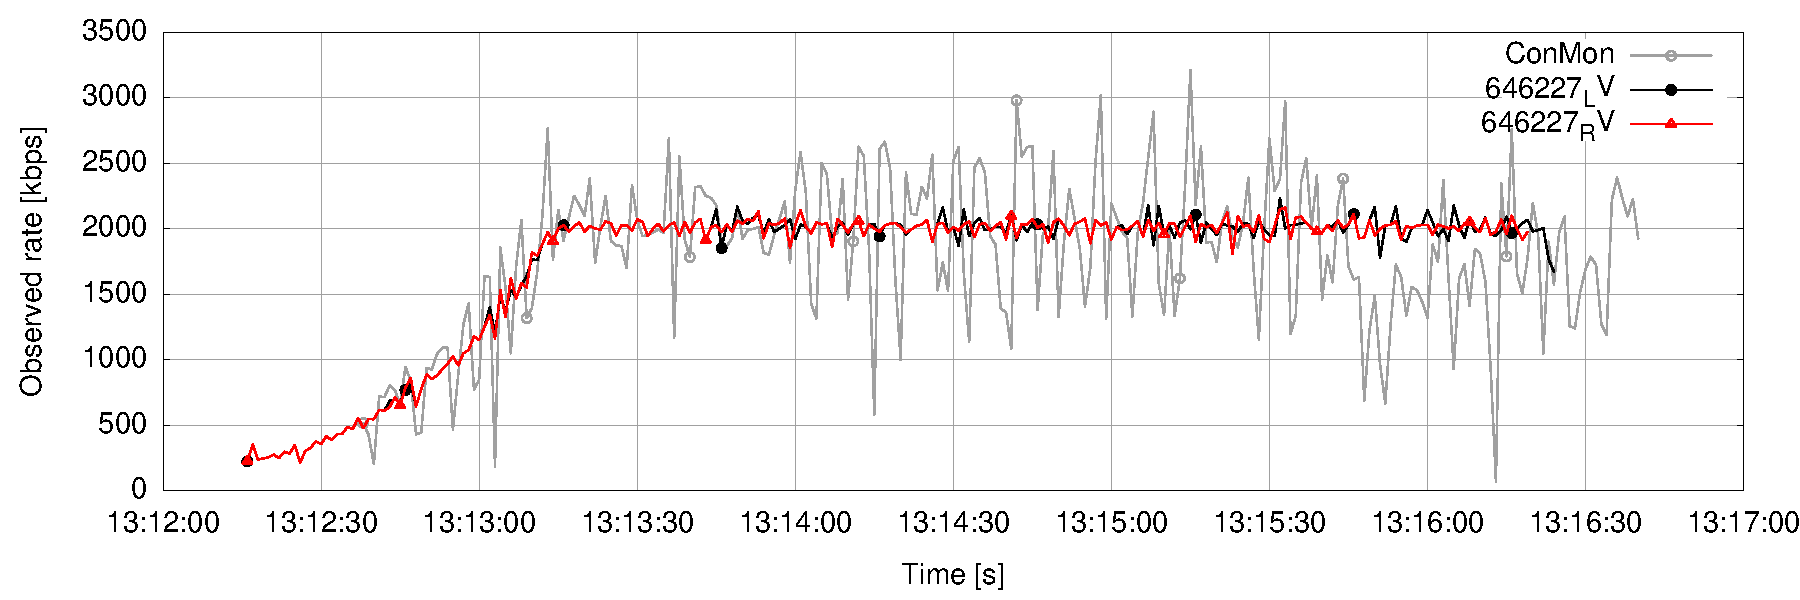
\includegraphics[width=1\textwidth]{./figures/onetoone_wifi_statsconmon.pdf}
      \caption[Point-to-point video stream plot using StatsAPI and ConMon data over WiFi]{Point-to-point video stream plot using StatsAPI and ConMon data over WiFi.}
	\label{fig:onetooneWifistatsconmon}
\end{figure}

Figure~\ref{fig:onetooneWifistatsconmon} represents the throughput rate on the same video stream, the three lines are the comparison between local video stream in origin peer, remote video stream in receiver peer and {\it ConMon} capture of the remote video stream on the receiver peer. All three streams contain the same data but they are measured in different layers, this will help us to understand the difference of throughput that is handling the overhead of the RTP and the disruption caused by the WiFi network.

Notice that red and black colors represent the Local Video (LV) and Remote Video (RV) from the same SSRC, both captures indicate the same stream captured using {\it StatsAPI}, and the grey line plots the capture performed using {\it ConMon} of the same SSRC. It is easy to observe that both {\it StatsAPI} captures are similar, some offset is produced due to the processing time between the network layer and the browser API that returns all values. Besides this, the capture is neat and throughput at the output of the origin client and input of the receiver is similar. Capture in the network layer is more abrupt as all packets are captured and the period of calculus when plotting affects when the value is added, when having two opposite values peaks they should be balanced, meaning that the transmission in most of the period is stable and the peaks when plotting are a result of accuracy. Call duration in this test has been around five minutes. Some areas, mostly between 13.15.30 and 13.16.00, show a strange behavior of the link that might be produced by the WiFi, this throughput distortion is balanced on the WebRTC layer as the throughput delivered by the API does not change.

When we try to measure the quality of the call one important indicator is the delay, to calculate the delay we can either use the RTT measured by our {\it StatsAPI} or use the captures performed on the network layer by {\it ConMon}. The {\it ConMon} procedure will give us a high accuracy on the delay subtracting both timestamps from both of the clients, this will require to reduce the drift of the internal clock of the computers.

 \begin{figure}[h]
  \centering
    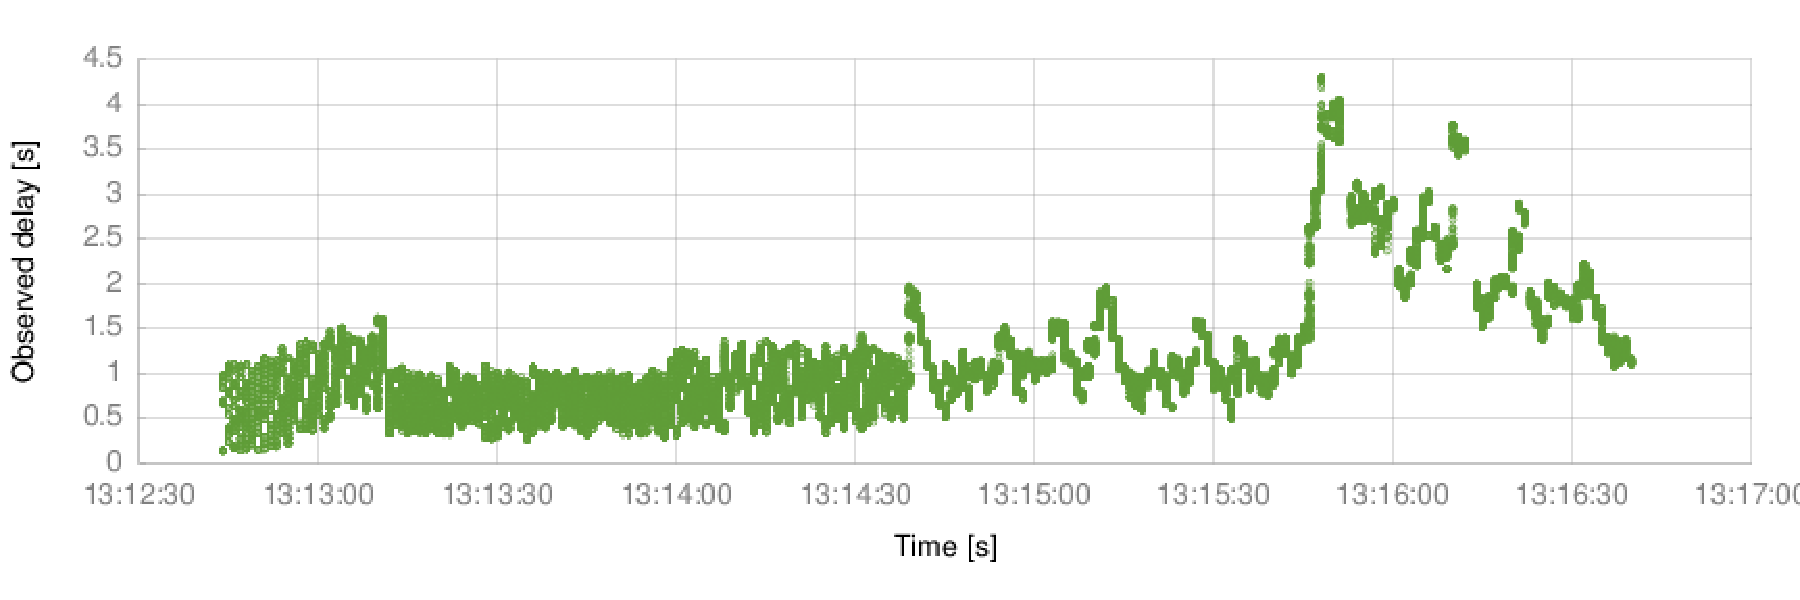
\includegraphics[width=1\textwidth]{./figures/delay_116_646227.pdf}
      \caption[Delay calculated on the same stream captured using ConMon in both ends over WiFi]{Delay calculated on the same stream captured using ConMon in both ends over WiFi.}
	\label{fig:delay_116_646227}
\end{figure}

Figure~\ref{fig:delay_116_646227} represents the delay of the stream plotted in~\ref{fig:onetooneWifistatsconmon}. We can see that the quality of the call is affected by the network distortion at the end of Figure~\ref{fig:onetooneWifistatsconmon}, this variation of the throughput delivers a high delay of more than 4 seconds during some period of time between 13:15:30 and 13:16:30, the media received at that time will not render correctly and the user experience of the call is going to be worst than at the beginning of the call. A bursty WiFi network will led to delay even the bandwidth seems to be stable.

\subsection{Different wired scenarios}

After seeing how WebRTC performs in WiFi  we are going to proceed with all tests in a controlled wired scenario adding different constraints to the link. This tests will be automated running ten iterations every time in order to get as much accurate results as possible.
 
 \begin{figure}[h]
  \centering
    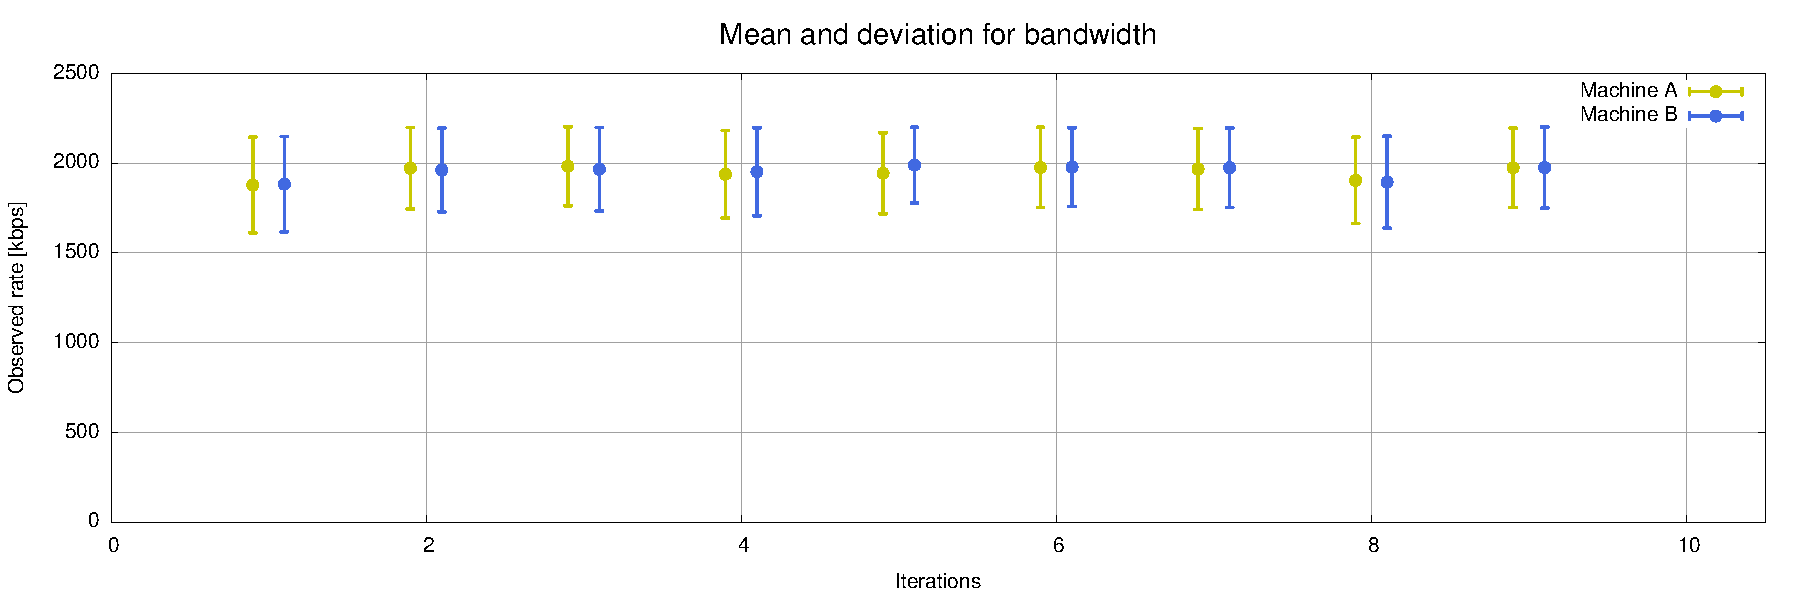
\includegraphics[width=1\textwidth]{./figures/no_ipfw.pdf}
      \caption[Bandwidth results for non-conditioned link]{Bandwidth results for non-conditioned link.}
	\label{fig:no_ipfw}
\end{figure}

Figure~\ref{fig:no_ipfw} plots the average bandwidth of every call in a wired network without any link condition, the average bandwidth obtained in the test is 1949.7 Kbit/s with 233 Kbit/s of deviation which gives the conclusion of having approximately 2 Mbit/s standard bandwidth in a video stream for a non-conditioned link in WebRTC. Delay result in 5.1 ms with 1.5 ms deviation and RTT about 9.5 ms. Those results can be taken as standard for a non-conditioned WebRTC with high bandwidth resources. A summary of results is shown in Table~\ref{fig:p2p_no_ipfw}. Some interesting results to track is the amount of calls failed in every test, considering all those calls go through a TURN server we might be able to approximate the success rate when establishing calls. All results go along with the deviation being this an important factor, in this test without any link conditioner we might have small deviation values such as milliseconds, but when adding conditions to the link those values will grow carrying less accuracy.
Setup time is stablished as the time it take since the start of the PeerConnection object until the media stream from the other peer arrives, this value directly affects the time it takes for a user to be able to start talking, in the optimal environment it takes about 1.5 seconds to start the call.

\begin{table}
\begin{center}
    \begin{tabular}{c D{,}{\pm}{-1} D{,}{\pm}{-1} D{,}{\pm}{-1} }
   	 \toprule
	\textit{}
	& \multicolumn{1}{c}{\textit{Machine A}}
	& \multicolumn{1}{c}{\textit{Machine B}}
	& \multicolumn{1}{c}{\textit{Overall}}\\
	\midrule
	\textbf{CPU (\%)} & 48.76 ,2.76 & 48.83 ,2.78 & 48.79 ,2.77\\
	\textbf{Memory (\%)} & 35.98 ,0.3 & 36.43 ,0.29 & 36.21 ,0.29\\
	\textbf{Bandwidth (Kbit/s)} & 1947.61 ,232.75 & 1951.76 ,234.5 & 1949.7 ,233.62\\
	\textbf{Setup time (ms)} & 1436.33 ,25 & 1447.44 ,22.71 & 1441.88 ,24.04\\
	\textbf{RTT (ms)} & 9.49 ,2.11 & 9.64 ,2.71 & 9.57 ,2.41\\
	\textbf{Delay (ms)} & 4.84 ,1.5 & 5.4 ,1.53 & 5.12 ,1.52\\
	\textbf{Losses (packets)} & 0 & 2 & 0.33\\
	\hline
	\textbf{Failed call} & & 2 &\\
	\bottomrule
    \end{tabular}
    \caption[P2P test with no link conditions]{P2P test with no link conditions.}
    \label{fig:p2p_no_ipfw}
\end{center}
\end{table}

Delay values in Table~\ref{fig:p2p_no_ipfw} are represented as a mean calculation of all the delay obtained in the link, thus this value is not representative of what happened in the call. Considering the example in Figure~\ref{fig:delay_116_646227} we can see that the delay can variate during the call being the mean not appropriate to measure the response against the conditions of the link. In order to observe the behavior of WebRTC in delay we have two different approaches, the mean delay with deviation and delay distribution of all calls.